\section{Discussion of results}

%\subsection{Symmetry suppression in pyramidal quantum dots}
%The suppression theory in \ref{sec:suppression} is discussed in the context of the quantum dots grown in the mode described in \ref{sec:growth}. The limiting symmetry of the nanocrystallic structure is shown. The effects of strain and other causes of perturbation are discussed. The $C_{3v}$ probing for the $X_{\bar{1},1}$ transition is discussed and explanations are offered.

\subsection{Agreement with the bulk symmetry $T_d$}
Observing which exciton complexes seem to elevate to $T_d$ generates predictions within our theory about the localisation of their wavefunctions within the QD bulk. The exciton transitions which were observed to undergo symmetry elevation to $T_d$ in the MCJP dataset are $X_{\bar{1}0}$ (for one sub-population), $X^-_{\bar{1}0}$ (not in the Karlsson data), $2X^+_{\bar{2}1}$ (with one peak being ambiguously identified to the transition), $X^+_{\bar{1}1}$ (for one sub-population),  $X^+_{1\bar{1}}$ (with the relative intensity of the polarisations not explicable with symmetry arguments), and $2X_{\bar{2}0}$ (assuming the $6$ lines are unresolvable due to tight spacing). Conversely, the excitons $X_{0\bar{1}}$ (for one sub-population), $X^+_{\bar{1}1}$ (for one sub-population), and $X^+_{1\bar{1}}$ (only in the Karlsson data) seem to explicitly disconfirm $T_d$ symmetry and probe for the structure symmetry. It is important to note that the sub-population divisions for the neutral excitons and for the positive excitons are different.

It seems that all excitons with only heavy holes undergo symmetry elevation to the bulk, in agreement with Sec. \ref{sec:localisation}. The ambiguity for mixed-hole excitons suggests that light holes indeed may probe the structure symmetry due to their delocalisation. Neither MCJP not Karlsson \textit{et al.} were able to resolve the light hole-dominant excitons for which the predictions of $C_{3v}$ and $T_d$ differ ($X^+_{0\bar{2}}$, $2X_{0\bar{2}}$, and positive biexcitons with $2$ or $3$ light holes). Resolving these transitions is important material for further study, since if they behave according to structure symmetry, it would be evidence that the symmetry suppression   model correctly identifies the mechanism for symmetry elevation.

Regarding the transition $X^+_{1\bar{1}}$ (Fig. \ref{fig:exciton_positive}), Karlsson \textit{et al.} have experimentally measured the fine-strucure energy splitting of the exciton complex $X^+_{11}$, ordering its corresponding energy levels labelled by their transformation properties \cite[p. 16]{karlsson}. In $C_{3v}$, the lowest and highest energy levels transform as $E_{3/2}$, and the middle two energy levels transform as $E_{1/2}$ \cite[Fig. 17]{karlsson}. This could explain the relative intensities of differently-polarised components of lines in the MCJP dataset, with the $z$-polarisation dominance in lines $c,b$ caused by the different transformation properties of their initial states compared to the initial states of lines $d,a$. It is possible that the wavefunction centre-localisation depends on the exciton transformation properties, affecting the magnitude of symmetry suppression enjoyed by specific lines.

\subsection{Possible sources of error from theoretical treatment and experimental setup}

In our treatment of the exciton envelope functions, we disregard band-mixing effects caused by the nanocrystal structure and small number of lattice points (Sec. \ref{sec:envelopes}). However, the pyramidal QDs subject to this study exhibit strong valence band mixing, which affects photoluminiscence polarisation \cite{strong_band_mixing}. This may affect the envelope function treatment, especially outside of the $\Gamma$ point, as it contradicts an assumption in the treatment. However, the effect the valence-band mixing has on photoluminiscence polarisation may also aid in explaining the relative intensities of the differently-polarised lines. A more mathematically robust treatment of envelope functions is crucial material for further study.

An important phenomenon disregarded in our treatment is the effect of structure interfaces, which affect the Hamiltonian symmetry group \cite{interfaces}. Whilst a full treatment of the symmetry suppression model has to address this to prove elevation to $T_d$ is still possible, this could also validate our data e.g. by providing the polarisation bias to $X^+_{1\bar{1}}$, explaining the relative line intensities.

Finally, for all transitions where we identify elevation to $T_d$, the main evidence consists of the increased number of $z$-polarised lines from the one predicted by $C_{3v}$ and $D_{3h}$. Hence our argumentation relies on the fact that these $z$-polarised components were identified correctly. However, if a physical effect unaccounted for in the experimental setup caused the reading of a non-zero $z$-polarised component where the emission has no $z$-polarised component, the measured $z$-polarised line would match the frequency of the measured $\sigma$-polarised line, analogously to how the non-polarised light predicted by $T_d$ produces lines of matching frequencies in both polarisations. This alternative explanation is supported by the apparent partial disagreement between the MCJP and Karlsson \textit{et al.} datasets specifically regarding the presence of $z$-polarised lines (Fig. \ref{fig:single_negative}, \ref{fig:biexciton_neutral}). In future study, careful reproduction of the $z$-polarised spectra for exciton complexes identified as elevating to bulk symmetry is crucial for disproving the symmetry suppression hypothesis.

\subsection{Insufficient treatment of line number increase} \label{sec:failed_degeneracy}
The model of symmetry suppression postulates that excitons with wavefunctions localised in the QD bulk enjoy approximate elevation to the bulk (lattice symmetry). Within this model, lines which are light in the lower symmetry but dark in the elevated symmetry will be heavily suppressed. However, the opposite effect (where the number of lines increases with symmetry elevation), which occurs for certain excitons when elevating to $T_d$, is non-trivial. This is because the increase of number of lines is often caused by the change of transformation properties of holes when the light hole band and heavy hole band become degenerate at $\Gamma$ (Table \ref{tab:multihole_states}). Within symmetry suppression theory, we consider the component of a low-symmetry eigenstate which forms an eigenstate of a high-symmetry Hamiltonian, but the residual component still demands different energy levels for the two hole types, suppressing the band distance but keeping it non-zero. For the model to be rigorous, additional treatment of this phenomenon must be introduced, either resolving the transformation properties of holes  under elevation to a group with the hole bands degenerate, or by identifying a mechanism that couples the different-character holes together, salvaging the degenerate behavour within our model. This is material for further study of symmetry elevation within the symmetry suppression framework.

\subsection{Symmetry outside of the $\Gamma$ point} \label{sec:symmetry_outside_gamma}
In the symmetry suppression model, we have assumed all excited fermions to have zero crystal momentum, which is necessary to use the ``charged particles in a box'' dynamics for the envelope functions. However, this is only an approximation based on the nature of the direct band-gap of InGaAs. For an excited fermion outside of the $\Gamma$ point in a large crystal, the non-zero crystal momentum vector $\vec{k}$ breaks the wavefunction symmetry, as described by Dresselhaus in \cite[Ch. 13]{dresselhaus}. In an interplay with the bulk symmetry, the true symmetry of the Hamiltonian $\hat{H}\left(\vec{k}\right)$ depends on the crystal momentum. 

In our nanocrystal, the effects of the crystal size alter the band structure, and a full description of the wavefunction is not possible with the crystal momentum, but rather with the shape of the envelope function, which is poorly understood. Exciting the envelope function from the ground state (i.e. leaving the $\Gamma$ point) may break some symmetries, but in general, it also changes the transformation properties of the wavefunction, since $\chi^{\left(\Upsilon\left(\vec{r}\right)\right)}\left(\hat{R}\right)$ in eq. \ref{eq:character_breakdown} is no longer always unity. This could potentially explain the division of QDs into two sub-populations for some exciton complexes (and the discrepancy with the Karlsson data), where the distribution of envelope function energies would become a non-trivial statistical phenomenon. However, the shapes of the envelope functions are not yet well understood, as they are highly sensitive to high-order or mechanical effects, such as strain-induced piezoelectricity (Fig. \ref{fig:lens_envelopes}).

Of course, since the extra degree of freedom in transformation properties could alter any prediction for photoluminiscence spectrum, it may also serve as an alternative explanation to symmetry elevation.\\

\makebox[0pt][l]{%
\begin{minipage}{\textwidth}
\centering
    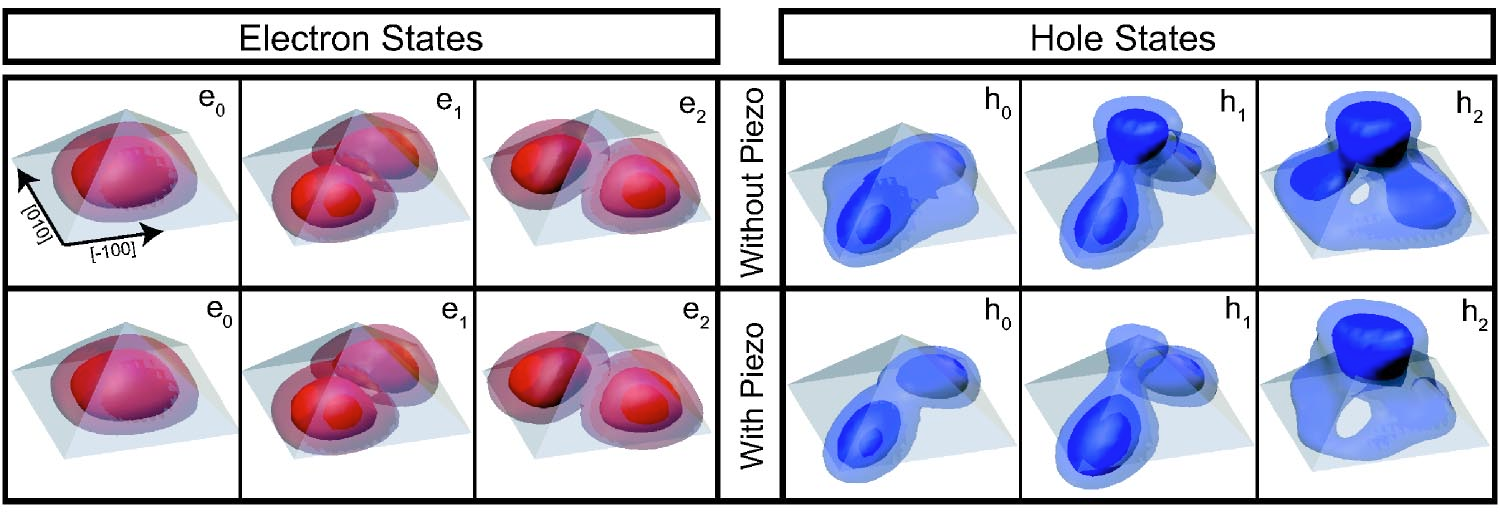
\includegraphics[width=\textwidth]{figures/pyramid_envelopes}
 \captionof{figure}{Envelope functions of ground- and excited-state electrons and holes in a $C_{4v}$ pyramid structure for first-order theory and including strain-induced piezoelectric effect. Figure taken from \cite[Fig. 6]{bulk_limiting}}
 \label{fig:lens_envelopes}
\end{minipage}
}